\lstset{language=VBScript,
        basicstyle=\footnotesize\ttfamily,
        breaklines=true,
        tabsize=2,
        numbers=left,
        numberstyle=\tiny,
        numbersep=7pt,
        showspaces=false,
        keywordstyle=\color{Blue}\textbf,
        commentstyle=\color{Red}\emph,
        showstringspaces=false,
        stringstyle=\color{BurntOrange}
        }
\section{Specyfikacja wewnętrzna}
%\subsection{Specyfikacja zewnętrzna}
Zaimplementowana przez autora wizualizacja ma na~celu zobrazowanie działania modelu oraz umożliwienie operatorowi 

Dodatkowo do~przycisków F9~-~F12 została przypisana zmiana stanu zmiennej \emph{EmergencyStop}, która pozwala na~awaryjne zatrzymanie pracy robota w~dowolnym momencie. Modyfikowanie wartości zmiennej odpowiadającej za~awaryjne zatrzymanie pracy może się również odbywać poprzez kliknięcie na~kontrolkę znajdującą się w~prawym dolnym rogu każdego ekranu.
Ekrany dostępne w wizualizacji oraz klawisze funkcyjne z nimi związane:
\begin{itemize} 
\item Ekran powitalny - F1,
\item Stan robota - F2,
\item Stan magazynu i testowanie obsługi - F3,
\item Testowanie sterowania ręcznego z pilota podłączonego do sterownika - F4,
\item Testowanie sterowania ręcznego z poziomu wizualizacji - F5,
\item Testowanie sterowania automatycznego - F6.
\end{itemize}
\indent
\indent Poszczególne ekrany zostaną szczegółowo opisane w kolejnych podrozdziałach.

\begin{figure}[!htb] 	
\centering 	
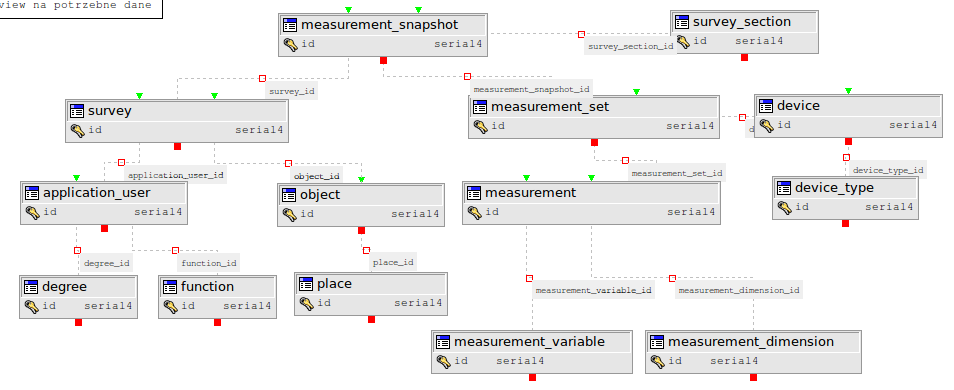
\includegraphics[width=0.95\textwidth]{images/database} 
\caption{Schemat bazy danych} 
\label{template}
 \end{figure}